\documentclass[tikz,border=2pt]{standalone}
\usepackage{tikz}
\usetikzlibrary{positioning}

\begin{document}
	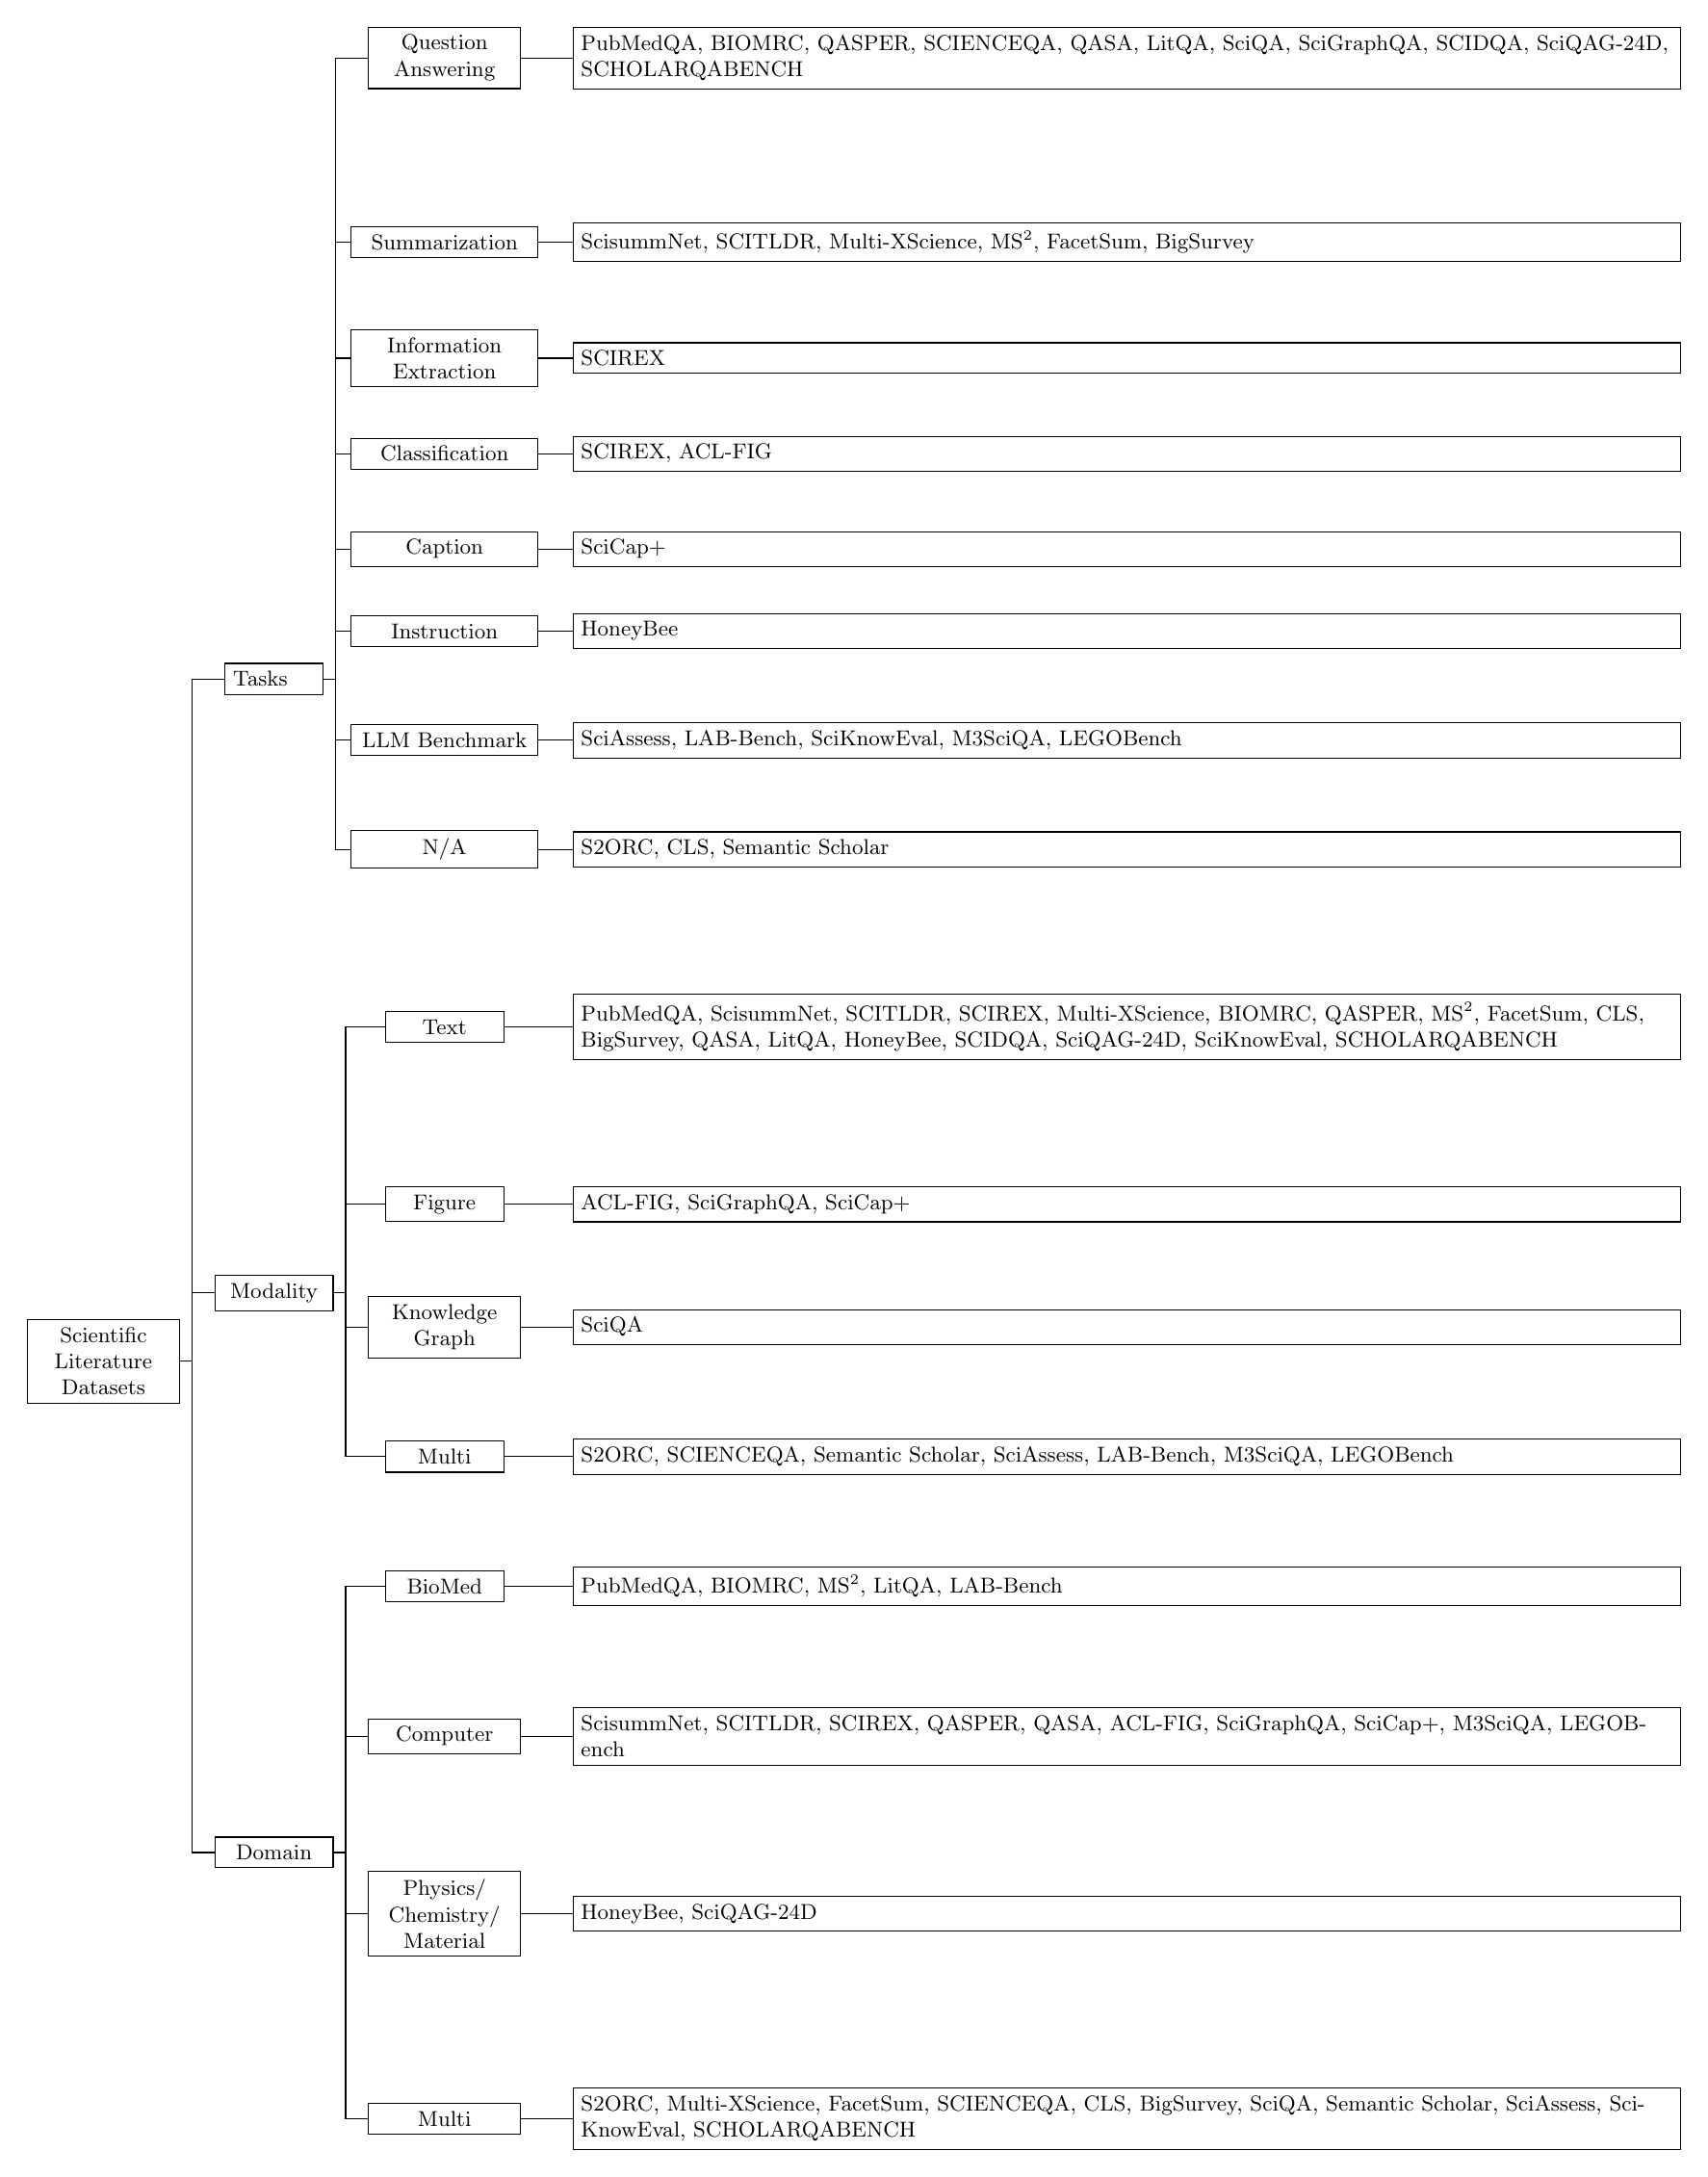
\begin{tikzpicture}[scale=0.9, transform shape,
		level distance=4cm,
		sibling distance=2cm,
		edge from parent path={(\tikzparentnode.east) -- ++(5pt,0) |- (\tikzchildnode.west)},
		every node/.style={draw, align=left, rectangle, minimum height=1em, font=\small},
		level 1/.style={level distance=2.5cm, sibling distance=10cm},
		level 2/.style={level distance=2.5cm, sibling distance=2.6cm},
		level 3/.style={level distance=10cm},
		grow'=right,
		]
		
		\node[text width=2cm, align=center] {Scientific Literature Datasets}
		child {node[text width=1.2cm] {Tasks}
			child {node[text width=2cm, align=center] {Question\\ Answering}
				child {node[text width=16cm] {PubMedQA, BIOMRC, QASPER, SCIENCEQA, QASA, LitQA, SciQA, SciGraphQA, SCIDQA, SciQAG-24D, SCHOLARQABENCH}}}
			child {node[text width=2.5cm, align=center, yshift=-0.1cm] {Summarization}
				child {node[text width=16cm] {ScisummNet, SCITLDR, Multi-XScience, MS\textsuperscript{2}, FacetSum, BigSurvey}}}
			child {node[text width=2.5cm, align=center, yshift=0.8cm] {Information\\ Extraction}
				child {node[text width=16cm] {SCIREX}}}
			child {node[text width=2.5cm, align=center, yshift=2cm] {Classification}
				child {node[text width=16cm] {SCIREX, ACL-FIG}}}
			child {node[text width=2.5cm, align=center, yshift=3.2cm] {Caption}
				child {node[text width=16cm] {SciCap+}}}
			child {node[text width=2.5cm, align=center, yshift=4.6cm] {Instruction}
				child {node[text width=16cm] {HoneyBee}}}
			child {node[text width=2.5cm, align=center, yshift=5.6cm] {LLM Benchmark}
				child {node[text width=16cm] {SciAssess, LAB-Bench, SciKnowEval, M3SciQA, LEGOBench}}}
			child {node[text width=2.5cm, align=center, yshift=6.6cm] {N/A}
				child {node[text width=16cm] {S2ORC, CLS, Semantic Scholar}}}
		}
		child {node[text width=1.5cm, align=center, yshift=1cm] {Modality}
			child {node[text width=1.5cm, align=center]{Text}
				child {node[text width=16cm]{PubMedQA, ScisummNet, SCITLDR, SCIREX, Multi-XScience, BIOMRC, QASPER, MS\textsuperscript{2}, FacetSum, CLS, BigSurvey, QASA, LitQA, HoneyBee, SCIDQA, SciQAG-24D, SciKnowEval, SCHOLARQABENCH}}}
			child {node[text width=1.5cm, align=center]{Figure}
				child {node[text width=16cm]{ACL-FIG, SciGraphQA, SciCap+}}}
			child {node[text width=2cm, align=center, yshift=0.8cm]{Knowledge\\ Graph}
				child {node[text width=16cm]{SciQA}}}
			child {node[text width=1.5cm, align=center, yshift=1.5cm]{Multi}
				child {node[text width=16cm]{S2ORC, SCIENCEQA, Semantic Scholar, SciAssess, LAB-Bench, M3SciQA, LEGOBench}}}
		}
		child {node[text width=1.5cm, align=center, yshift=2.8cm] {Domain}
			child {node[text width=1.5cm, align=center]{BioMed}
				child {node[text width=16cm]{PubMedQA, BIOMRC, MS\textsuperscript{2}, LitQA, LAB-Bench}}}
			child {node[text width=2cm, align=center, yshift=0.4cm]{Computer}
				child {node[text width=16cm]{ScisummNet, SCITLDR, SCIREX, QASPER, QASA, ACL-FIG, SciGraphQA, SciCap+, M3SciQA, LEGOBench}}}
			child {node[text width=2cm, align=center, yshift=0.4cm]{Physics/\\Chemistry/\\Material}
				child {node[text width=16cm]{HoneyBee, SciQAG-24D}}}
			child {node[text width=2cm, align=center]{Multi}
				child {node[text width=16cm]{S2ORC, Multi-XScience, FacetSum, SCIENCEQA, CLS, BigSurvey, SciQA, Semantic Scholar, SciAssess, SciKnowEval, SCHOLARQABENCH}}}
		};
	\end{tikzpicture}
\end{document}
